\documentstyle[times,art10,twocolumn,latex8,graphics]{article}
%\documentclass[times,art10,twocolumn,latex8]{article}

%\usepackage[dvips]{graphicx}
%\usepackage[pdftex]{graphicx}
%\usepackage[pdftex]{graphics}

\begin{document}
% \pagestyle{empty}
% totalnumber=4


\title{High-Performance Quasi Double-Precision Method using Single-Precision \\
       Hardware for Molecular Dynamics Simulations with GPUs}

\author{Tetsu Narumi$^1$\\
narumi@a7.keio.jp \\
% For a paper whose authors are all at the same institution, 
% omit the following lines up until the closing ``}''.
% Additional authors and addresses can be added with ``\and'', 
% just like the second author.
\and
Tsuyoshi Hamada$^2$\\
hamada@cis.nagasaki-u.ac.jp\\
\and
Keigo Nitadori$^3$\\
nitadori@astron.s.u-tokyo.ac.jp\\
\and
Ryuji Sakamaki$^1$\\
sakamaki@atwired.com\\
\and
Shun Kameoka$^1$\\
fsharpminor@a2.keio.jp\\
\and
Kenji Yasuoka$^1$\\
yasuoka@mech.keio.ac.jp\vspace*{3mm}\\
\and
$^1$Department of Mechanical Engineering, Keio University \\
3-14-1 Hiyoshi, Kohoku, Yokohama 223-8522, JAPAN\vspace*{3mm}\\
$^2$Department of Computer and Information Sciences, Nagasaki University\\
1-14 Bunkyo Machi, Nagasaki, 852-8521, JAPAN\vspace*{3mm}\\
$^3$Department of Astronomy, University of Tokyo\\
7-3-1 Hongo, Bunkyo-ku, Tokyo 113-0033, JAPAN
}
\maketitle
% \thispagestyle{empty}


\begin{abstract} The recent advancement of computer technology in 
commodity hardware enables us to perform scientific simulations on
them.  For example, the Cell processor in the PLAYSTATION 3 (PS3) has
a 179 Gflops peak performance in single precision, which exceeds the
fastest CPU for PCs.  Moreover, GeForce GTX280, the latest Graphics
Processing Unit (GPU) by NVIDIA, has 933 Gflops peak performance in
single precision. However, the double precision performance of these
computers is not so good: a PS3 has 17 Gflops and a GTX280 has 78
Gflops, which is comparable to current CPUs for PCs. Using
mixed-precision arithmetic is the key to extract the potential of
these hardware. In this paper, a new algorithm to use mixed-precision
arithmetic for the accumulation part of forces in Molecular Dynamics
(MD) simulations is proposed. The algorithm achieves comparable
accuracy to that of double precision with single-precision hardware by
quasi double-precision method.  Especially, no offset of accumulated
forces is the key feature of the method, which enhance the stability
of the MD simulation.  The speed of the quasi double-precision
calculation is in between those of double and single precisions.
\end{abstract}

%\begin{keywords} 
%molecular dynamics simulation, Graphics Processing Unit, PLAYSTATION 3,
%special-purpose computer, GRAPE
%\end{keywords}

%\begin{AMS}
% N-body problems, Simulation, Biophysics
%70F10, 68U20, 92C05
%\end{AMS}

%\pagestyle{myheadings}
%\thispagestyle{plain}

%\markboth{T. NARUMI, R. SAKAMAKI, S. KAMEOKA, and K. YASUOKA}
%{Overheads in Accelerating MD Simulations with GPUs}

\section{Introduction}\label{sec:introduction}

Precision of arithmetic operations in computer simulation is one of
the crucial issues for obtaining reasonable results.  However, during
the past decade most simulations have used the double precision as a
default since it is usually accurate enough, and CPUs perform double
precision arithmetic operations with similar performance to single
precision.  One exceptional case is when you use a short vector,
Single Instruction Multiple Data (SIMD) unit, such as Streaming SIMD
Extensions (SSE) in x86 CPU or AltiVec in PowerPC CPU.  For this case,
the calculation speed of single precision is twice as fast as that of
double precision with these units.

In the past two or three years, some processors having completely
different performances for different precisions have been developed.
For example, the Cell processor \cite{cell} in PLAYSTATION 3 (PS3)
\cite{PS3} has a 179 Gflops single precision peak performance, and
only 17 Gflops in double precision. GeForce GTX280, the latest GPU
from NVIDIA \cite{NVIDIA}, has 933 Gflops single precision
performance, and only 78 Gflops in double precision. Though the single
precision performances of these processors exceed the latest Intel
CPU, such as Xeon X7460 (128 Gflops) \cite{XeonX7460}, the double
precision performance is comparable to the CPU (64 Gflops).  In order
to achieve maximum performance on these processors, it is necessary to
use as many single precision arithmetic operations as possible.  The
challenge in using single precision operations is the reduction of
round-off errors in the calculation results.  Using mixed-precision
arithmetic operations is a promising approach to achieve high
performance and high accuracy at the same time.

Buttari et al. \cite{Buttari} used mixed-precision for performing
matrix operations.  In the iterative loop for solving matrix
equations, they used single precision operations for the most
computationally heavy parts.  Other parts are performed with double
precision because higher accuracy is required for assuring the
convergence of the iterative solution.  By using this technique, they
achieved the same results as the double precision with much higher
performance on the Cell processor. 

MD simulation is a powerful technique to investigate the physical
property of condensed mater at an atomic level \cite{Karplus}. Atoms
in a system interact with each other via the Coulomb, van der Waals,
and bonding forces. Among these forces, two body interactions with the
Coulomb and van der Waals forces are dominant when the number of atoms
in a system becomes large. Therefore the computational cost of MD
simulations can become overwhelming for large systems.  To enhance the
performance of the MD simulation code, many techniques have been used
on the basis of mixed-precision. For example, GROMACS \cite{GROMACS},
one of the fastest MD simulation codes with a single thread, uses SSE
unit in Intel CPUs to enhance the performance. NAMD \cite{NAMD1,
NAMD2}, one of the fastest parallel MD codes, supports GPU to enhance
the performance. In both codes, the two body force calculations are
performed in single precision to extract the maximum performance of
the hardware.

In spite of the previous efforts of single precision force calculation
on GPUs \cite{NAMD1, NAMD2, GPUneighbor}, the accumulation of forces
is not performed accurate enough, because the hardware did not support
double precision at that time.  Since summing up many forces from
surrounding atoms with single precision operations often cause a
rounding off error \cite{Hamada2}, a more accurate precision, such as
double precision, should be used.  Takahashi et al. \cite{Takahashi1,
Takahashi2} used a mixed-precision for accelerating the boundary
element method with a GPU. Nitadori \cite{Nitadori} and Hamada et
al. \cite{Hamada1} also used mixed-precision for gravitational
$N$-body simulations with a GPU. Both of them achieved quasi
double-precision by using a pair of single-precision variables to
increase the accuracy at the force accumulation part.

In this paper we propose a new method to perform the accumulation of
forces with comparable accuracy to double precision using
single-precision hardware, and the speed of the method is in between
those of double and single precisions.
In section \ref{sec:quasidouble}, the previous idea of using quasi
double-precision is described. In section \ref{sec:propose}, the
proposed method is explained in detail. The accuracy and the
performance of the method are presented in section
\ref{sec:numerical}. In section \ref{sec:conclude}, summary and
comments are shown.

\section{Quasi Double-Precision Method}\label{sec:quasidouble}

In this section, the method to increase the accuracy of 
summation is described. Here, we concentrate on the situation
that a single precision value is added to an accumulated value, 
which is expressed in various formats.

\subsection{Error in floating point expression}

When a number, $x$, is expressed by a floating point value, $fl(x)$,
the following condition is satisfied,
\begin{equation}
\frac{fl(x)}{x}<2^{-n},
\end{equation}
where $n$ denotes the number of mantissa bits including a hidden bit.
This equation shows the range of the error of the floating point 
expression.
If the double and single precision expression of $x$ 
is expressed as $fl_D(x)$ and $fl_S(x)$ respectively, the errors in 
these expressions are:
\begin{eqnarray}
\frac{fl_D(x)}{x} &<& 2^{-n_D}\simeq 10^{-16},\\
\frac{fl_S(x)}{x} &<& 2^{-n_S}\simeq 10^{-7},
\end{eqnarray}
since the number of mantissa bits of double and single precision
are $n_D=53$ and $n_S=24$ respectively in the IEEE754 standard.
$10^{-7}$ error of single precision is often insufficient for 
target applications. One easy solution is to use double precision, 
but the other is to use multiple single precision variables to express 
one value. We will use $x_D$ or $x_S$ 
instead of $fl_D(x)$ or $fl_S(x)$ hereafter for simplicity.

\subsection{Knuth \& Dekker's trick}

Knuth \cite{Knuth} and Dekker \cite{Dekker}
proposed a method to sum two values without
losing so much accuracy. If two single precision values, 
$x_S$ and $y_S$, satisfy $|x_S|\geq |y_S|$, their sum 
can be expressed by the following expression:
\begin{equation}
x_S + y_S = z_S + zz_S,
\end{equation}
where $z_S$ and $zz_S$ are:
\begin{eqnarray}
z_S &=& fl_S(x_S + y_S),\nonumber \\
w_S &=& fl_S(z_S - x_S),\label{eqn:KaD1}\\
zz_S &=& fl_S( y_S - w_S).\nonumber
\end{eqnarray}
Here $fl_S(x+y)$ and $fl_S(x-y)$ denote the single precision floating point 
addition and subtraction respectively.
$z_S$ and $zz_S$ can be understood as the higher and lower part
of the result respectively, as they satisfy the following equation:
\begin{equation}
|\frac{z_S}{zz_S}|<2^{-n_S}.
\end{equation}
In the following paper, we call this combination of 
higher and lower expressions a {\it pair expression}.
The error in the {\it pair expression}, $2^{-2 n_S}=2^{-48}\simeq 10^{-15}$,
is comparable to double precision and much lower than single precision.
Figure \ref{fig:KaD1} shows the program for Equation (\ref{eqn:KaD1})
in C language. Here '{\tt SS z}' is a variable for a {\it pair 
expression}: ${\tt z.hs}=z_S$ and ${\tt z.ls}=zz_S$.

Dekker also proposed a modified method which does not need the
condition, $|x_S|\geq |y_S|$, as follows:
\begin{eqnarray}
z_S &=& fl_S(x_S + y_S),\nonumber \\
w_S &=& fl_S(z_S - x_S),\nonumber \\
z1_S &=& fl_S(y_S - w_S),\nonumber \\
v_S &=& fl_S(z_S - w_S),\label{eqn:KaD2}\\
z2_S &=& fl_S(v_S - x_S),\nonumber \\
zz_S &=& fl_S(z1_S - z2_S).\nonumber
\end{eqnarray}
Figure \ref{fig:KaD2} shows the program for Equation (\ref{eqn:KaD2}).


\begin{figure}
\begin{center}\footnotesize
\begin{minipage}{100mm}\def\baselinestretch{0.8}
\begin{verbatim}
 1 typedef struct {
 2     float hs;
 3     float ls;
 4 } SS;
 5 
 6 SS add_knuth_and_dekker1(float xs, float ys)
 7 {
 8     float ws;
 9     SS z;
10 
11     z.hs = xs   + ys;
12     ws   = z.hs - xs;
13     z.ls = ys   - ws;
14 
15     return z;
16 }
\end{verbatim}\def\baselinestretch{1.0}
\end{minipage}
\caption{Knuth \& Dekker's trick in C language when $|x_S|\geq |y_S|$.}
\label{fig:KaD1}
\end{center}
\end{figure}

\begin{figure}
\begin{center}\footnotesize
\begin{minipage}{100mm}\def\baselinestretch{0.8}
\begin{verbatim}
 1 SS add_knuth_and_dekker2(float xs, float ys)
 2 {
 3     float ws, vs, z1s, z2s;
 4     SS z;
 5 
 6     z.hs = xs   + ys;
 7     ws   = z.hs - xs;
 8     z1s  = ys   - ws;
 9     vs   = z.hs - ws;
10     z2s  = vs   - xs;
11     z.ls = z1s  - z2s;
12 
13     return z;
14 }
\end{verbatim}\def\baselinestretch{1.0}
\end{minipage}
\caption{Knuth \& Dekker's trick in C language for arbitrary $x_S$ and $y_S$.}
\label{fig:KaD2}
\end{center}
\end{figure}

\subsection{Takahashi \& Iitaka's trick}

Knuth \& Dekker's trick is often used when much more accuracy is
required than the hardware supported precision. One example is the
DSFUN90 library \cite{highprecisionlib} which uses multiple
single-precision arithmetic.  Knuth \& Dekker's trick has already been
used on GPUs.  In this paper, we refer to Takahashi \& Iitaka's trick
\cite{Takahashi1, Takahashi2}.

The target problem is to sum up single precision values into
an accumulated value. Here we assume that 
we already have an accumulated value
by a {\it pair expression}, $a_S$ and $aa_S$, where $a_S$ and $aa_S$
are the higher and lower part of the accumulated result respectively.
Then the summation of $y_S$ and a {\it pair expression} of $a_S$ and $aa_S$
are performed by the following procedure in Takahashi \& 
Iitaka's trick.
\begin{equation}
a_S + y_S + aa_S = b_S + bb_S,
\end{equation}
where
\begin{eqnarray}
z_S  &=& fl_S( a_S + y_S ),\nonumber \\
w_S  &=& fl_S( z_S - a_S ),\nonumber \\
z1_S &=& fl_S( y_S - w_S ),\nonumber \\
v_S  &=& fl_S( z_S - w_S ),\nonumber \\
z2_S &=& fl_S( v_S - a_S ),\nonumber \\
zz_S &=& fl_S( z1_S - z2_S ),\label{eqn:TaI}\\
r_S  &=& fl_S( aa_S + zz_S ),\nonumber \\
b_S  &=& fl_S( z_S  + r_S  ),\nonumber \\
t_S  &=& fl_S( b_S  - z_S  ),\nonumber \\
bb_S &=& fl_S( r_S  - t_S  ),\nonumber 
\end{eqnarray}
%
% forcef[k] -> a_S, b_S, forcef2[k] -> aa_S, bb_S, dr[k] -> y_S
% force2f[k] second time -> r_S, w second time -> t_S

Figure \ref{fig:TaI} shows their method in C language, 
which requires 10 operations (3 summations and 7 subtractions).
Here '{\tt SS a}' holds a {\it pair expression} of $a_S$ and $aa_S$,
and '{\tt SS b}' does of $b_S$ and $bb_S$.

Their method can be rewritten by using Knuth \& Dekker's trick
as shown in Figure \ref{fig:TaI2}.
The method is composed of three parts.
In the first part (line 6 in Figure \ref{fig:TaI2}),
Knuth \& Dekker's trick (\ref{eqn:KaD2}) is used.
In the second part (line 7 in Figure \ref{fig:TaI2}), 
lower part of {\it pair expressions} are added with each other.
In the third part (line 8 in Figure \ref{fig:TaI2}),
the method expressed in Equation (\ref{eqn:KaD1}) can be used.
The reason is that $|z_S|\geq |r_S|$ is satisfied
since $r_S$ is the sum of the lower part of {\it pair expressions}
and $z_S$ is the higher part.


\begin{figure}
\begin{center}\footnotesize
\begin{minipage}{100mm}\def\baselinestretch{0.8}
\vspace*{-3mm}
\begin{verbatim}
 1 SS add_takahashi_and_iitaka(SS a, float ys)
 2 {
 3   float ws, vs, z1s, z2s, rs, ts;
 4   SS z, b;
 5 
 6   z.hs = a.hs + ys;
 7   ws   = z.hs - a.hs;
 8   z1s  = ys   - ws;
 9   vs   = z.hs - ws;
10   z2s  = vs   - a.hs;
11   z.ls = z1s  - z2s;
12   rs   = a.ls + z.ls;
13   b.hs = z.hs + rs;
14   ts   = b.hs - z.hs;
15   b.ls = rs   - ts;
16 
17   return b;
18 }
\end{verbatim}\def\baselinestretch{1.0}
\end{minipage}
\caption{Takahashi \& Iitaka's trick in C language.}
\label{fig:TaI}
\end{center}
\end{figure}

\section{High-Performance Quasi Double-Precision Method}\label{sec:propose}

In this section, a proposed method for accumulating forces with
quasi double-precision is presented. 

\subsection{Nitadori's trick}

We have proposed a simplified method, Nitadori's trick
\cite{Nitadori}, where only 4 operations are needed per summation,
while Takahashi \& Iitaka's trick costs 10 operations.  Figure
\ref{fig:Nitadori1} shows the program in C language.

In the method, two conditions are assumed. The first condition is that
the accumulated value should be larger than a value which is going to
be added. Therefore, the method of Equation (\ref{eqn:KaD1}) can be
used instead of Equation (\ref{eqn:KaD2}). The other condition is that
the target application should not be sensitive to the small decrease
of the accuracy in a {\it pair expression}.  For example, when 128
values are added to the accumulated value by this method, the lower
part becomes larger and larger.  Then the error in the {\it pair
expression} is in the worst case 128 times larger than $2^{-48}$,
which is the normal accuracy of the single precision {\it pair
expression}. When larger number of values are added, much larger error
might be generated by this method. However in collision-less $N$-body
simulation, the error does not seem to be a problem
\cite{Hamada1}. For other gravitational $N$-body simulations, detailed
analysis will be presetnted elsewhere.  In the MD simulation,
this error has a notable effect in some cases.

\subsection{Modified Nitadori's trick}

Figure \ref{fig:Nitadori2} shows the program to calculate a force
({\tt fd}) by accumulating {\tt nj} pairwise forces ({\tt fs}) with
Nitadori's trick. 
When {\tt LARGE} is set to {\tt 0.0}, the first
condition of the Nitadori's trick must be satisfied to obtain the
correct result. This means that the absolute value of the accumulated
value must be larger than that of each force ($|{\tt a[k].hs}|\geq |{\tt
fs[k]}|$). However, when {\tt LARGE} is set to be a large number,
such as {\tt (3<<20)}$\simeq 3 \times 10^6$, the first condition is
always satisfied as each force is always smaller than {\tt
LARGE}. Note that if {\tt LARGE} is set too large, the
accuracy of the accumulation becomes lower because of the rounding
off. We call this method modified Nitadori's trick. 

A sample code to calculate pairwase force is shown in Figure \ref{fig:calcvdw}.
In the actual code used in Section \ref{sec:numerical}, 
each particle has its own atom type and it is highly optimized to the GPU.
{\tt calcvdw} is a sample code to show how to call accumulation
routine.

\begin{figure}
\begin{center}\footnotesize
\begin{minipage}{100mm}\def\baselinestretch{0.8}
\vspace*{-3mm}
\begin{verbatim}
 1 SS add_takahashi_and_iitaka(SS a, float ys)
 2 {
 3   float rs;
 4   SS z, b;
 5 
 6   z  = add_knuth_and_dekker2(a.hs, ys);
 7   rs = a.ls + z.ls;
 8   b  = add_knuth_and_dekker1(z.hs, rs);
 9 
10   return b;
11 }
\end{verbatim}\def\baselinestretch{1.0}
\end{minipage}
\caption{Takahashi \& Iitaka's trick in C language with Knuth \& Dekker's subroutines.}
\label{fig:TaI2}
\end{center}
\end{figure}

\begin{figure}
\begin{center}\footnotesize
\begin{minipage}{100mm}\def\baselinestretch{0.8}
\vspace*{-4mm}
\begin{verbatim}
 1 SS add_nitadori(SS a, float ys)
 2 {
 3     SS b;
 4 
 5     b    = add_knuth_and_dekker1(a.hs, ys);
 6     b.ls = a.ls + b.ls;
 7 
 8     return b;
 9 }
\end{verbatim}\def\baselinestretch{1.0}
\end{minipage}
\caption{Nitadori's trick in C language with Knuth \& Dekker's subroutines.}
\label{fig:Nitadori1}
\end{center}
\end{figure}

\begin{figure}
\begin{center}\footnotesize
\begin{minipage}{100mm}\def\baselinestretch{0.8}
\begin{verbatim}
 1 #if 1 // change to 0 for modified Nitadori's 
 2       // and Narumi's methods
 3 #define LARGE        0.0f
 4 #else
 5 #define LARGE_SHIFT  21
 6 #define LARGE  \
 7         (float)(3 << (LARGE_SHIFT-1))
 8 #endif
 9 
10 void accumulate_nitadori(float ri[3], 
11        float rj[][3], int nj, double fd[3])
12 {
13   int j, k;
14   SS a[3];
15   float fs[3];
16 
17   for(k=0; k<3; k++){
18     a[k].hs = LARGE;
19     a[k].ls = 0.0f;
20   }
21   for(j=0; j<nj; j++){
22     pairwiseforce(ri, rj[j], fs);
23     for(k=0; k<3; k++){
24       a[k] = add_nitadori(a[k], fs[k]);
25     }
26   }
27   for(k=0;k<3;k++){
28     fd[k]  = a[k].hs - LARGE;
29     fd[k] += a[k].ls;
30   }
31 }
\end{verbatim}\def\baselinestretch{1.0}
\end{minipage}
\caption{Accumulation of forces by Nitadori's trick.
For modified Nitadori's trick, line 1 must be 
changed from {\tt \#if 1} to {\tt \#if 0},
and {\tt LARGE\_SHIFT} must be set to a large enough 
number to satisfy {\tt LARGE}$\geq |${\tt fs[k]}$|$.}
\label{fig:Nitadori2}
\end{center}
\end{figure}

\begin{figure}
\begin{center}\footnotesize
\begin{minipage}{100mm}\def\baselinestretch{0.8}
\begin{verbatim}
 1 void pairwiseforce(float ris[3], float rjs[3], 
 2                    float fs[3])
 3 {
 4   int k;
 5   float ds[3], rs, qs, ps;
 6 
 7   for(k=0; k<3; k++) ds[k] = ris[k] - rjs[k];
 8   rs = ds[0]*ds[0] + ds[1]*ds[1] + ds[2]*ds[2];
 9   if(rs != 0.0f){
10     rs = 1.0f / rs;
11     qs = rs * rs * rs;
12     ps = rs * qs * (2.0f * qs - 1.0f);
13     for(k=0; k<3; k++) fs[k] = ps * ds[k];
14   }
15   else{
16     for(k=0; k<3; k++) fs[k] = 0.0f;
17   }
18 }
19 
20 void calcvdw(int ni, int nj, float ri[][3], 
21              float rj[][3], double fd[][3])
22 {
23   int i;
24 
25   for(i=0; i<ni; i++){
26     accumulate_nitadori(ri[i], rj, nj, fd[i]);
27     // accumulate_narumi(ri[i], rj, nj, fd[i]);
28   }
29 }
\end{verbatim}\def\baselinestretch{1.0}
\end{minipage}
\caption{Calculatioin of van der Waals forces with
(modified) Nitadori's method.}
\label{fig:calcvdw}
\end{center}
\end{figure}

\subsection{Proposed method : Narumi's trick}

Figure \ref{fig:Narumi} shows the proposed method expressed by C language.
This method is based on the Nitadori's trick but 
prevents the second condition in the Nitadori's trick.

First, quasi double-precision struct, {\tt SI}, is defined. This struct houses
a single precision value ({\tt float hs}) and a 32-bit integer ({\tt int li}).
{\tt hs} and {\tt li} correspond to the higher and lower part of a {\it pair
expression} respectively.
{\tt LOWER\_FACTOR} is the factor to be multiplied to a floating point
value to convert it to an integer.
{\tt LOWER\_FACTOR\_1} is the factor to be multiplied to an integer
to convert it back to floating point expression.

{\tt LOWER\_SHIFT} specifies the number of bits to be set 0 at
the MSBs (Most Significant Bits) of the lower part of a {\it pair
expression} ({\tt li}). The preceding 0s guarantee the non-overflow of
{\tt li} even when {\tt add\_narumi} is called 128 (={\tt
  LOWER\_LOOP}={\tt 1<<LOWER\_SHIFT}) times. The reason for
using 32-bit integers instead of single precision is that 32-bit
integers have more resolution compared to single precision when a
decimal point is fixed. Because of this expression, even when the
ratio between the higher and lower part of the {\it pair expression} is
changed, the accuracy of accumulation does not decrease as in the
Nitadori's trick.

\begin{figure}
\begin{center}\footnotesize
\begin{minipage}{100mm}\def\baselinestretch{0.8}
\vspace*{-2mm}
\begin{verbatim}
 1 typedef struct {
 2     float hs;
 3     int   li;
 4 } SI;
 5 
 6 #define LOWER_SHIFT  7
 7 #define LOWER_LOOP   (1 << LOWER_SHIFT)
 8 #define LOWER_FACTOR   \
 9         (float)(1LL << (23 - LARGE_SHIFT \
10                       + 32 - LOWER_SHIFT))
11 #define LOWER_FACTOR_1 \
12         ( 1.0f / LOWER_FACTOR ) 
13 #define MASK(n)          ((0x1<<(n)) -1)
14 
15 SI add_narumi(SI a, float ys)
16 {
17   SS b;
18   SI c;
19   
20   b    = add_knuth_and_dekker1(a.hs, ys);
21   c.hs = b.hs;
22   c.li = a.li+(int)(b.ls * LOWER_FACTOR);
23   
24   return c;
25 }
26  
27 void accumulate_narumi(float ri[3], 
28        float rj[][3], int nj, double fd[3])
29 {
30   int j, jj, k;
31   SI a[3];
32   float fs[3];
33 
34   for(k=0; k<3; k++){
35     a[k].hs = LARGE;
36     a[k].li = 0;
37   }
38   for(jj=0; jj<nj; jj+=LOWER_LOOP){
39     for(j=jj;j-jj<LOWER_LOOP && j<nj;j++){
40       pairwiseforce(ri, rj[j], fs);
41       for(k=0; k<3; k++){
42         a[k] = add_narumi(a[k], fs[k]);
43       }
44     }
45     for(k=0; k<3; k++){
46       a[k].hs += (float)(a[k].li & 
47        (MASK(LOWER_SHIFT)<<(32-
48        LOWER_SHIFT)))*LOWER_FACTOR_1;
49       a[k].li &= MASK(32-LOWER_SHIFT);
50     }
51   }
52   for(k=0; k<3; k++){
53     fd[k] = a[k].hs - LARGE;
54     fd[k]+= a[k].li * (double)LOWER_FACTOR_1;
55   }
56 }
\end{verbatim}\def\baselinestretch{1.0}
\end{minipage}
\caption{Accumulation of forces by proposed method.
{\tt LARGE} is set to be a large enough number to
satisfy $|{\tt a[k].hs}|\geq |{\tt fs[k]}|$. {\tt LOWER\_SHIFT}
is set to such as 7 to prevent the second condition
of Nitadori's trick.}
\label{fig:Narumi}
\vspace*{-4mm}
\end{center}
\end{figure}

\begin{figure}
\begin{center}
\resizebox{8.5cm}{!}{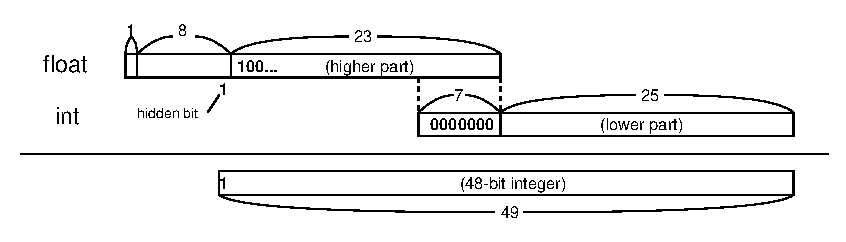
\includegraphics{figure/narumiblock.eps}}
\caption{Block diagram of a {\it pair expression} in Narumi's trick.
A {\tt float} and an {\tt int} are used, and they correspond to
a 48-bit integer.}
\label{fig:narumiblock}
\vspace*{-5mm}
\end{center}
\end{figure}


\subsection{Accuracy of Narumi's trick}

Figure \ref{fig:narumiblock} shows the block diagram of the {\it pair
expression} of Narumi's trick. The reason {\tt LARGE} is set to {\tt
  3<<20} instead of {\tt 1<<21} is that the position of a decimal point 
and the sign are fixed for $|{\tt fs[k]}|<${\tt (1<<20)}. With this method 
the decimal points of the higher and lower part of the {\it pair 
expression} are fixed, which means that the {\it pair expression} is 
equivalent to a 48-bit integer as shown in Figure\ref{fig:narumiblock}. 
The accuracy of the {\it pair expression} is$2^{-48}\simeq 10^{-15}$, 
which is the same as the Takahashi \&Iitaka's trick. Note that, similar 
to the modified Nitadori's trick, the accuracy becomes lower when {\tt 
LARGE} is large compared to each force.

\subsection{Number of operations in Narumi's trick}

The number of operations per summation is 6 in Narumi's trick. 3 is
used for Knuth \& Dekker's trick.  3 is for the line 22: {\tt
  c.li=a.li+(int)(b.ls * LOWER\_FACTOR)}.  The
multiplication in this line can be deleted when each force is already
multiplied by changing parameters to be {\tt LOWER\_FACTOR} times
larger. The conversion from {\tt float} to {\tt int} also takes one
operation. The operations in the lines 46-49 are negligible since these
lines are performed every {\tt LOWER\_LOOP} times.  Therefore, the
total number of operations per a summation is 5 instead of 4 in the
Nitadori's trick or 10 in the Takahashi \& Iitaka's trick.  When {\tt
  LOWER\_LOOP} is small ({\tt LOWER\_SHIFT} is small), the
operations for lines 46-49 has some impact on the performance.



\section{Numerical Test}\label{sec:numerical}

In the following part, numerical error analysis of the proposed method 
is presented. Then its performance is described.

\subsection{Test systems}

Two systems are used to numerically test the proposed method.  One is
a protein system (System 1), which is used for testing accuracy.
The other is a simple system with Lennard Jones particles (System 2),
which is used for performance benchmark.  For both systems, only the
two body interaction of the van der Waals force is evaluated without
cutoff.  Other forces, such as the Coulomb and bonding forces, are not
calculated.  When the two body interaction is calculated on a
molecule, forces on the bonded part on the molecule are skipped.  One
way to do this, is to mask the bonded interaction in the force
summation loop. One needs to check the mask bit in the most internal
loop, which causes a performance drop since the mask bit differs for
each thread.  Another way is to first calculate the two body
interaction on all combinations in a system and then subtract the
bonded part afterwards.  The first one is called 'Exclude on the fly'
and the other is called 'Exclude afterwards', in this paper.
'Exclude on the fly' algorithm is used in NAMD with GPU \cite{NAMD1}.

System 1 contains a protein, Scytalone dehydratase (2,715 atoms), and
208 water molecules.  Total number of atoms is 3,339, and AMBER
\cite{AMBER} force field is used to calculate the forces on atoms.
System 2 contains 65,536 particles, and 
16 atom types are randomly assigned to each particle.
Parameters for the Lennard Jones potential are also randomly generated.
Note that atom types and these parameters do not influence the
performance.
Exclusion of the bonded part is not needed.



\subsection{Average error in force}

Figure \ref{fig:aef} shows the average error of forces for the 
various methods.
Methods are summarized in Table \ref{tbl:method}.
The average error of forces is calculated as follows:
\begin{equation}
f_{\rm err} = \frac{ \sum_{i=1}^{N} | \vec F_{{\rm method}_i} - \vec F_{{\rm double}_i}|}
              { \sum_{i=1}^{N} | \vec F_{{\rm double}_i}|},
\end{equation}
where $\vec F_{{\rm double}_i}$ is the force on the $i$-th particle with full double precision
calculation (method G), $\vec F_{{\rm method}_i}$ is the force of a specified method,
and $N$ is the total number of particles in the system.
The average error of forces is similar when the 'Exclude on the fly'
algorithm is used. As shown in our previous paper \cite{PS3Narumi},
average error of forces of $10^{-3}$ or larger is not sufficient for
a stable MD simulation. Therefore, methods A and D are not useful
with the 'Exclude afterwards' algorithm.

\begin{figure}
\begin{center}
\vspace*{-2mm}
\resizebox{7cm}{!}{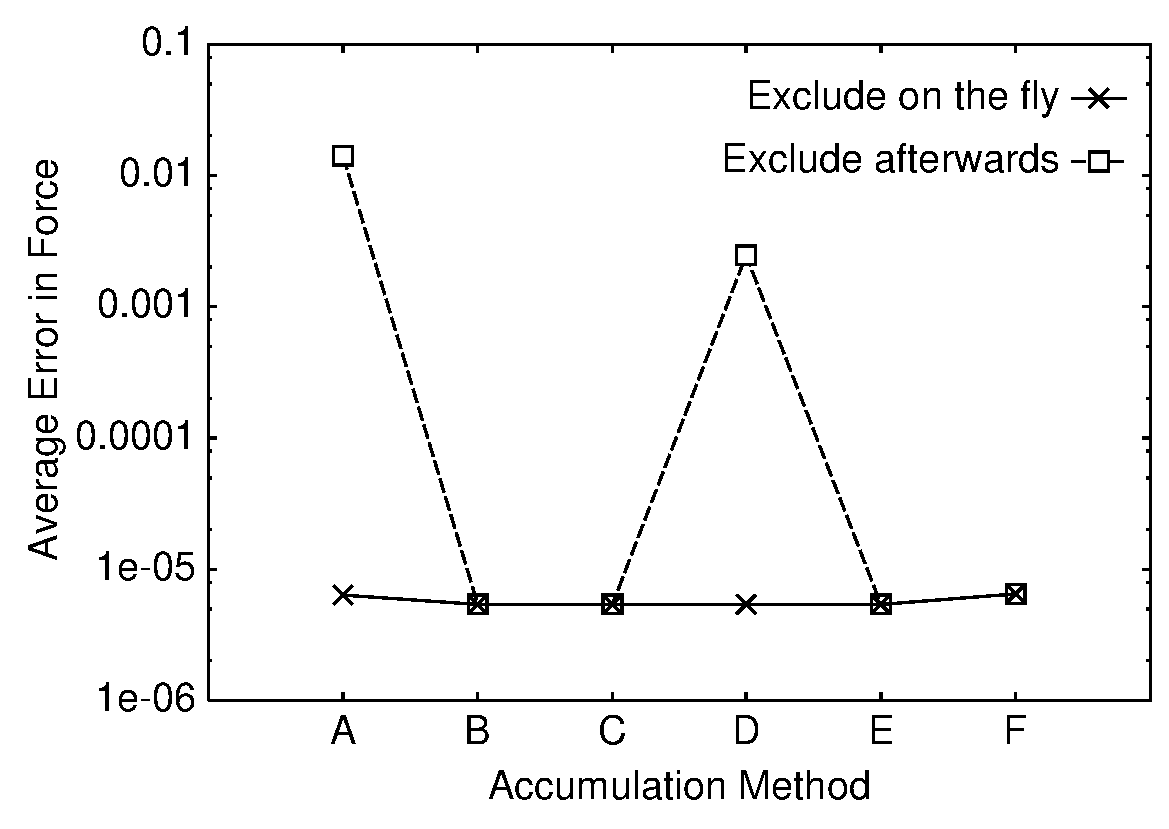
\includegraphics{figure/afe.eps}}
\caption{Average error of forces for System 1 against accumulation methods.}
\label{fig:aef}
\vspace*{-3mm}
\end{center}
\end{figure}


\subsection{Average offset in force}

Figure \ref{fig:aof} shows the average offset of forces
against various methods. Methods are summarized in Table \ref{tbl:method}.
Average offset of forces is calculated as follows:
\begin{equation}
f_{\rm offset} = \frac{ | \sum_{i=1}^{N} \vec F_{{\rm method}_i} | }
                 { \sum_{i=1}^{N} | \vec F_{{\rm method}_i} | }.
\end{equation}
The numerator of the equation, sum of forces, should be zero if there
is no numerical error in the calculation because of the Newton's third
law.  The average offset of forces is important for the stability of the
time integration of the particle positions. If there is a big offset in
the forces, it means the Newton's third law is not satisfied, and the
energy in the system tends to increase even for the microcanonical
ensemble. The microcanonical ensemble should keep the total energy in
the system fixed in the range of the numerical error because no additional
energy is introduced in the system.  With the 'Exclude on the fly'
algorithm, methods B, C, D, F, and G satisfy the sufficiently small
offset in forces, while with the 'Exclude afterwards' algorithm, only
methods B, C, F, and G satisfy this condition.  
Note that the proposed method F has
no offset in forces, while the method G with full double precision has some
offset.  This is why the proposed method uses fixed point instead of
floating point. Fixed point guarantees the arbitrary order of summation
for the same result.

\subsection{Performance}

Figure \ref{fig:perf} shows the calculation speed (number of pairwise
interaction per second) of van der Waals forces with 9800GTX and 
GTX280 GPUs with different types of methods shown in Table
\ref{tbl:method}. Method B is not applicable to 9800GTX because it
doesn't support double precision.  For this performance benchmark, a
relatively large system is calculated without cutoff though usual MD
simulation for Lennard Jones particles uses a cutoff to reduce the
calculation cost.  The reason is to remove as many overheads as
possible to measure the speed for the internal of the force
calculation loop with different accumulation methods.

The proposed method F is faster than the method B, which is the 
accumulation with
double precision. Method F is slightly slower than Nitadori's
method D. These results show that the double precision support of the
latest GPU is not so useful for van der Waals calculations since the
method F can be executed without double precision.


\begin{figure}
\begin{center}
\vspace*{-3mm}
\resizebox{7cm}{!}{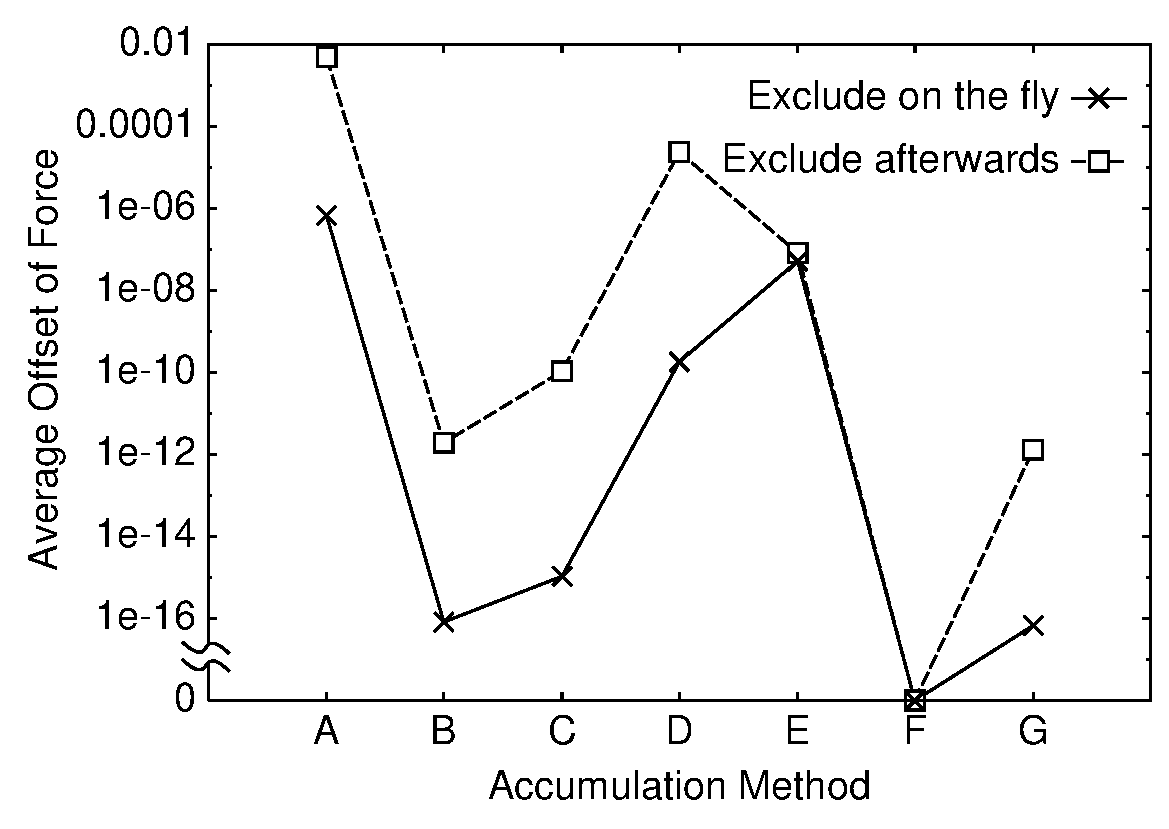
\includegraphics{figure/aof.eps}}
\caption{Average offset of forces for System 1 against accumulation methods.
Proposed method F has no offset.}
\label{fig:aof}
\end{center}
\end{figure}

\begin{figure}
\begin{center}
\vspace*{-5mm}
\resizebox{7cm}{!}{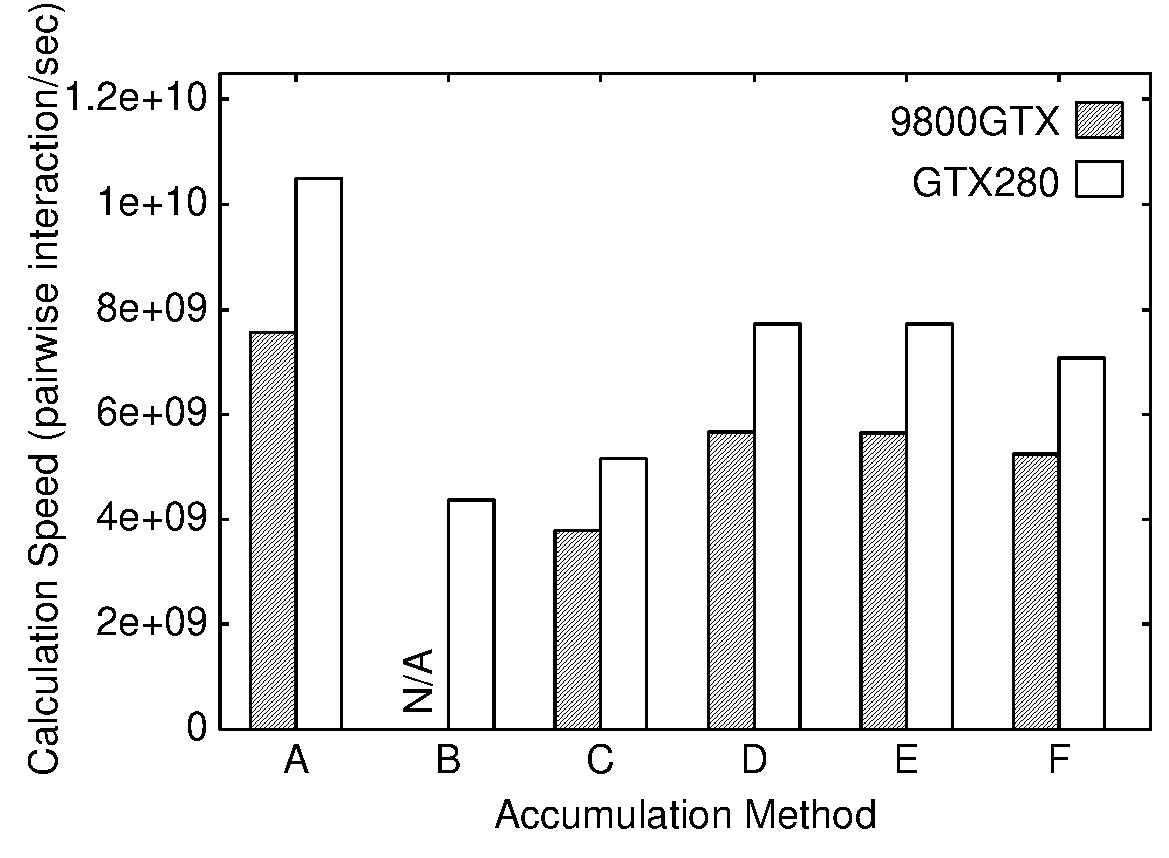
\includegraphics{figure/perf.eps}}
\caption{Performance of 9800GTX and GTX280 GPUs for van der Waals force
  calculation for System 2 with different types of methods. 
  Proposed method F is faster than the method B,
  accumulation with double precision.}
\label{fig:perf}
\vspace*{-5mm}
\end{center}
\end{figure}

\begin{table}
\caption{Accumulation methods}\label{tbl:method}
\begin{center}\footnotesize
\begin{tabular}{|c|l|l|}
\hline
Method & \multicolumn{1}{c|}{Pairwise force} 
       & \multicolumn{1}{c|}{Accumulation} \\
\hline
\hline
A & Single precision & Single precision \\
\hline
B & Single precision & Double precision \\
\hline
C & Single precision & Takahashi \& Iitaka's trick \\
\hline
D & Single precision & Nitadori's trick \\
\hline
E & Single precision & Modified Nitadori's trick \\
\hline
F & Single precision & Proposed method (Narumi's trick) \\
\hline
G & Double precision & Double precision\\
\hline
\end{tabular}
\vspace*{-3mm}
\end{center}
\end{table}

\section{Concluding Remarks}\label{sec:conclude}

The proposed method (Narumi's trick) has an accuracy equivalent to
that of a double precision calculation for the summation part
with single-precision hardware.
Notably, there are no offset in forces for the proposed method.  There
is no difference in the accuracy with 'Exclude on the fly' and
'Exclude afterwards' algorithms for the proposed method.  This is
useful for achieving high performance on the GPU, since the force
calculation part becomes simple when the 'Exclude afterwards'
algorithm is used.  For example, we can divide the force calculation
into two parts: two body interaction with GPU and exclusion on CPU. As
the exclusion part is not so heavy but a little complicated compared
with the two body interaction, the CPU is suitable for calculating it.
The two body interaction part without exclusion is simple and easy to
accelerate on the GPU. Therefore, the proposed method would be useful
for the actual MD codes on GPUs in the near future in terms of both
performance and accuracy.

\section*{Acknowledgement} 
Part of this study was supported by the Core 
Research for Evolution Science and Technology (CREST) of the Japan 
Science and Technology Corporation (JST)
and by the Ministry of Education, Science, Sports, and Culture,
Grant-in-Aid for Young Scientists (B), H20, 2070031.

% \setlength{\itemsep}{10pt}
\begin{thebibliography}{10}
{\small
\bibitem{cell} {\sc D. Pham, S. Asano, M. Bolliger, M.~N. Day,
H.~P. Hofstee, C. Johns, J. Kahle, A. Kameyama, J. Keaty,
Y. Masubuchi, M. Riley, D. Shippy, D. Stasiak, M. Suzuoki, M. Wang,
J. Warnock, S. Weitzel, D. Wendel, T. Yamazaki, K. Yazawa}, {\em The
design and implementation of a first-generation CELL processor}, in
Proceedings of Solid-State Circuits Conference, 1, (2005),
pp~184--592.\vspace*{-1mm}
\bibitem{PS3}
{\tt http://www.playstation.com/} (Oct. 2008).\vspace*{-1mm}
\bibitem{NVIDIA}
{\tt http://www.nvidia.com/} (Oct. 2008).\vspace*{-1mm}
\bibitem{XeonX7460}
{\tt http://www.intel.com/products/ processor/xeon7000/} (Oct. 2008).\vspace*{-1mm}
\bibitem{Buttari} Alfredo Buttari, Jack Dongarra, Julie Langou, Julien
  Langou, Piotr Luszczek, Jakub Kurzak, ``Mixed Precision Iterative
  Refinement Techniques for the Solution of Dense Linear Systems'',
  {\it International Journal of High Performance Computing
    Applications}, 21, (2007), pp~457-466.\vspace*{-1mm}
\bibitem{Takahashi1} Toru Takahashi, ``Hardware Acceleration for
  Boundary Element Methods'', Harvard/Riken GPGPU Symposium 2008,
  Cambridge, US, (Mar. 2008).\vspace*{-1mm}
\bibitem{Takahashi2} Toru Takahashi and Kazuki Koketsu, ``A high
performance computing using graphics boards in boundary element
methods'', in Proceedings of Keisan-Kougaku-Kouenkai, vol. 11, Osaka,
Japan, (Jun. 2006; in Japanese).\vspace*{-1mm}
\bibitem{Hamada1} T. Hamada, ``Simulation of Stellar Systems with
  GPUs'', {\it in Proceedings of the Forum on Advanced Scientific
    Simulation - Astrophysics}, Fukuoka, Japan, (2008), {\tt
    http://onokoro.cc.kyushu-u.ac.jp/forum08/ talk/Hamada.pdf}
  (Oct. 2008; in Japanese).\vspace*{-1mm}
\bibitem{Karplus} {M. Karplus and J. A. McCammon}, ``Molecular
dynamics simulations of biomolecules'', {\it Nat. Struct. Biol.}, 9,
(2002), pp~646-52.\vspace*{-1mm}
\bibitem{GROMACS} {\sc D. Van Der Spoel, E. Lindahl, B. Hess,
G. Groenhof, A.~E.  Mark, and H.~J. Berendsen} {\em Gromacs: fast,
flexible, and free}, J. Comput. Chem., 26 (16), (2005), pp~1701--1718.\vspace*{-1mm}
\bibitem{NAMD1} {J. E. Stone, J. C. Phillips, P. L. Freddolino,
D. J. Hardy, L. G. Trabuco, and K. Schulten}, ``Accelerating molecular
modeling applications with graphics processors'', {\it Journal of
Computational Chemistry}, 28, (2007), pp~ 2618-2640.\vspace*{-1mm}
\bibitem{NAMD2} {C. I. Rodrigues, D. J. Hardy, J. E. Stone,
K. Schulten, and W. W. Hwu}, ``GPU acceleration of cutoff pair
potentials for molecular modeling Applications'', {\it in Proceedings
of the 2008 Conference on Computing Frontiers}, (2008), pp~273-282.\vspace*{-1mm}
\bibitem{GPUneighbor}
{J. A. Anderson, C. D. Lorenz, and A. Travesset},
"General purpose molecular dynamics simulations fully implemented
on graphics processing units",
{\it Journal of Computational Physics}, 227, 10, (2008), pp~ 5342-5359.\vspace*{-1mm}
\bibitem{Hamada2} {T. Hamada and T. Iitaka}, ``The Chamomile Scheme:
An optimized algorithm for $N$-body simulations on programmable
graphics processing units'', {\it ArXiv Astrophysics e-prints},
astro-ph/073100, (2007).\vspace*{-1mm}
\bibitem{Knuth} {D. E. Knuth}, {\it The art of computer programming,
volume 2: seminumerical algorithms}, Addison-Wesley (1969).\vspace*{-1mm}
\bibitem{Dekker} {T. J. Dekker}, ``A floating-point technique for
extending the available precision'', {\it Numer. Math.}, 18 (1971),
pp~224-242.\vspace*{-1mm}
\bibitem{highprecisionlib} David H. Bailey, Yozo Hida, Karthik
Jeyabalan, Xiaoye S. Li, and Brandon Thompson, ``High-Precision
Software Directory'', {\tt http://crd.lbl.gov/\~{}dhbailey/ mpdist/}
(Oct. 2008).\vspace*{-1mm}
\bibitem{Nitadori} {K. Nitadori}, ``High-accuracy $N$-body simulations
on GPU'', {\it Poster in AstroGPU 2007}, Princeton, (2007).\vspace*{-1mm}
\bibitem{AMBER} {D.~A. Case, T.~A. Darden, T.~E. Cheatham III,
C.~L. Simmerling, J. Wang, R.~E. Duke, R. Luo, K.~M. Merz, B. Wang,
D.~A. Pearlman, M. Crowley, S. Brozell, V. Tsui, H. Gohlke, J. Mongan,
V. Hornak, G. Cui, P. Beroza, C. Schafmeister, J.~W. Caldwell,
W.~S. Ross, P.~A. Kollman}, {Amber 8.0}, University of California San
Francisco (2004).\vspace*{-1mm}
\bibitem{PS3Narumi} {T. Narumi, S. Kameoka, M. Taiji, and K. Yasuoka},
``Accelerating molecular dynamics simulations on PLAYSTATION 3 using
'Virtual-GRAPE' programming model'', {\it SIAM Journal on Scientific
Computing}, in press.\vspace*{-1mm}
}
\end{thebibliography}





\end{document}
